\Section{Cargo parancsok hívása a programból}

\begin{figure}[h!]
    \centering
    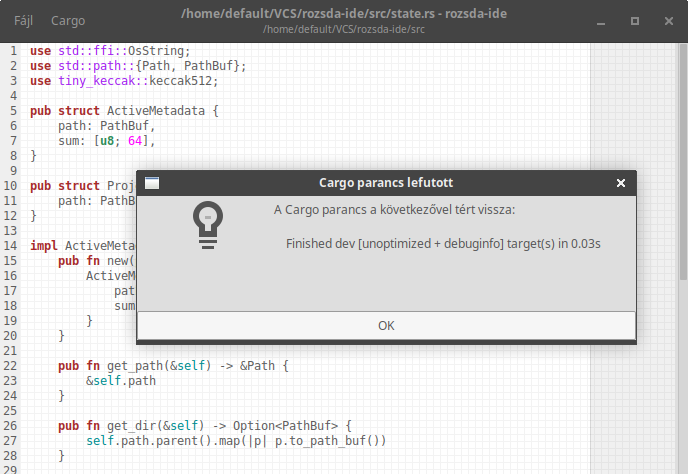
\includegraphics[width=0.8\textwidth]{cargo}
	\caption{Példa egy Cargo parancs futtatására}
	\label{fig:cargo_window}
\end{figure}

Egy fejlesztői környezethez viszont nem elégséges az, hogy megtudunk nyitni fájlokat,
és azokat tudjuk szerkeszteni.
A következőekben átrendezzük a programot, hogy azt tovább tudjuk bővíteni,
majd létrehozunk egy rendszert, amivel a Cargo segítségével kezelhetjük az éppen
megnyitott ládánkat.

Mint azt a kép is mutatja, egy célunk az lesz, hogy a Rozsda IDE-t saját magában
tudjuk nem csak szerkeszteni, de még lefordítani és futtatni is.

\SubSection{Menük behozatala és a \texttt{Header} struktúra átrendezése}

Mivel eddig csak egyszerű fájlkezelést hajtottunk végre, a fájlmegnyitást és -mentést
három gombbal hajtottuk végre, amit a fejlécen helyeztünk el.
Viszont ahogy növekednek a műveletek, amiket szeretnénk az IDE-vel végrehajtani,
ez a megoldás nem előnyös.

Mivel logikailag a fejléc alá rendeltek, így létrehozzuk a 
\texttt{ui/header/file\_menu.rs} és a \texttt{ui/header/cargo\_menu.rs} fájlokat.
Mindkét esetben létrehozunk egy saját struktúrát, ami felépíti egy menünek a tartalmát,
és ezeket a \texttt{Header}-ben egy \texttt{MenuBar}-ba helyezzük.
Fontos továbbá, hogy a menüelemek publikusak legyenek, mivel az \texttt{App} majd
eseményeket rendel hozzájuk.

\lstinputlisting[firstline=3, lastline=12, language=Rust]{./kodreszletek/11_cargo.rs}

A \texttt{Header}-t ezek után tovább módosítjuk.
Az eddigiekben a különféle fájlkiíró és -betöltő metódusok kaptak egy referenciát a
\texttt{HeaderBar}-ra, hogy annak a címét és alcímét módosíthassák.
Ugyan priváttá nem tehetjük a \texttt{HeaderBar}-t, mivel az \texttt{App}-nak szüksége
van egy referenciára rá, hogy a program ablakának fejlécévé tegye,
a \texttt{\&HeaderBar}-t igénylő metódusokat módosítjuk úgy, hogy ne kérjenek referenciát,
és így ne is módosítsák -- a cím és alcím módosítását a \texttt{Header}-re hagyjuk.

Ehhez először adattagként megadjuk az \texttt{ActiveMetadata}-t.

\lstinputlisting[firstline=18, lastline=24, language=Rust]{./kodreszletek/11_cargo.rs}

Illetve definiálunk a \texttt{Header}-nek egy saját metódust, ami csak azért felelős,
hogy a fejléc tartalmát módosítsa, majd a későbbiekben ezt hívjuk meg fájlműveletek után.

\lstinputlisting[firstline=30, lastline=32, language=Rust]{./kodreszletek/11_cargo.rs}

Ennek a metódusnak megadunk egy \texttt{same\_sum} paramétert, ami igaz,
hogy ha a háttértáron lévő fájl tartalma megegyezik a kódszerkesztő pufferével.
A fejléc tartalmának elkészítése ilyen módon megengedi nekünk, hogy a kódszerkesztő \texttt{changed}
jelzését kihasználva értesítsük a felhasználót arról, hogy mentetlen változásai vannak
(emlékezzünk, ezt a jelzést már használtuk a hash szummák összehasonlítására).

\SubSection{Projektkezelés}

Ahhoz, hogy Cargo parancsokat tudjunk végrehajtani egy ládán, amiben dolgozunk,
el kell tárolnunk a megadott láda elérési útvonalát.
Szerencsére ehhez hasonló feladatunk már volt az \texttt{ActiveMetadata} elkészítésénél,
így annak mintájára létrehozzuk a \texttt{ProjectMetadata} struktúrát a \texttt{state.rs} fájlban.

\lstinputlisting[firstline=45, lastline=47, language=Rust]{./kodreszletek/11_cargo.rs}

Ez továbbá sokkal egyszerűbb is logikailag, mint az \texttt{ActiveMetadata},
hiszen ebben az esetben egy könyvtár elérési helyét tároljuk el, és mi magunk műveleteket
nem hajtunk rajta végre, így elég csak két metódust létrehoznunk hozzá:
\texttt{get\_path()}, ami visszatér a teljes, abszolút elérési útvonallal,
és \texttt{get\_name()}, ami a könyvtár nevével.

A megadott láda kiválasztásához továbbá létrehozunk két újabb felugró ablakot,
szintúgy a létezőek mintájára.

\lstinputlisting[firstline=38, lastline=39, language=Rust]{./kodreszletek/11_cargo.rs}

Ezek megint nem térnek el sokban egymástól, és a már meglévő \texttt{FileChooserDialog} becsomagoló struktúráktól,
a legnagyobb különbség bennük a becsomagolt felugró ablak típusa 
(az újak esetén \texttt{SelectFolder} és \texttt{CreateFolder}).

A fájlválasztó felugró ablakok esetén továbbá létrehozunk egy szűrőt,
amit beállítunk úgy, hogy csak a Rust forrásfájlokat engedje megnyitni.

\lstinputlisting[firstline=130, lastline=134, language=Rust]{./kodreszletek/11_cargo.rs}

\SubSection{A \texttt{misc.rs} kibővítése}

Az \texttt{App} leegyszerűsítése, és az új követelmények kielégítése érdekében a \texttt{ui/misc.rs}
fájlt teljesen átdolgozzuk: mivel már a fejléc kezelése a \texttt{Header} feladata,
így azt a metódust eltávolítjuk, a fájlkezelési metódusokat átmozgatjuk ide az \texttt{App}-ból,
és új metódusokat hozunk létre a láda kezelési funkciókhoz.

\lstinputlisting[firstline=63, lastline=79, language=Rust]{./kodreszletek/11_cargo.rs}

Lehetőséget adunk a fájl bezárására a nélkül, hogy a felhasználónak be kellene zárnia az egész programot.
Viszont ekkor felléphet az a helyzet, hogy a felhasználó még nem mentette a változtatásait,
így az \texttt{ask\_about\_unsaved\_changes()} metódusban létrehozunk egy felugró ablakot,
ami felhívja a felhasználó figyelmét erre, ha szükséges.

Mint az \texttt{ActiveMetadata} esetében, a projektkezelő metódusok nagyban hasonlítanak a fájlkezelőkre,
kivéve, hogy nincs tartalom, amit kezelni kellene.
Egy nagy különbség viszont az, hogy egy projekt akkor tekinthető Cargo ládának, hogy ha létezik a
könyvtárában egy \texttt{Cargo.toml} fájl, így projekt megnyitáskor ellenőrizzük azt.

Végül az \texttt{App}-ban kihozzuk a jelenlegi fájlt (és projektet) adattagként, 
ezáltal leegyszerűsítve a metódus hívásokat, illetve egy \texttt{Arc}-ba csomagoljuk
a \texttt{Header}-t, ezáltal elérést biztosítva az azt érintő jelzéseknek --
egy jelzés meghívhat több metódust is aktiválásakor.

\lstinputlisting[firstline=109, lastline=116, language=Rust]{./kodreszletek/11_cargo.rs}

Az új műveleteket aktiváltatjuk a különféle menü elemek \texttt{connect\_activated()} jelzéseivel,
illetve létrehozunk új billentyű-kombinációkat a leggyakoribb műveletek meghívására is.
Jelenleg a programban a következő billentyű-kombinációk léteznek:

\begin{itemize}
    \item \texttt{F11}: Teljes képernyő
    \item \texttt{Ctrl+O}: Megnyitás
    \item \texttt{Ctrl+S}: Mentés
    \item \texttt{Ctrl+W}: Jelenlegi fájl bezárása
    \item \texttt{Ctrl+Q}: Program bezárása
\end{itemize}

\SubSection{Cargo parancsok}

A Cargo parancsoknak létrehozunk egy \texttt{cargo.rs} fájlt, amibe minden általunk használt
parancsnak létrehozunk egy metódust.
Ezek a \texttt{init --bin}, \texttt{init --lib}, \texttt{build}, \texttt{run}, \texttt{check}, \texttt{test} és \texttt{clean}.

A parancsok meghívásához a \texttt{Command} struktúrát használjuk, ami gyermekprocesszként elindítja a Cargo-t.
A metódusok általános formája a következő:

\lstinputlisting[firstline=51, lastline=58, language=Rust]{./kodreszletek/11_cargo.rs}

A kimenetet rövid formában kérjük minden esetben, ahol lehet.
Enélkül a kimenet \texttt{human} formában történik, ami terminálban történő megjelenítésre alkalmas.
Létezik még a \texttt{json} kimeneti forma is, viszont mi egyelőre csak tovább akarjuk adni a kimenetet
a felhasználónak anélkül, hogy azt feldolgoznánk -- így a \texttt{short} megfelel.

Az \texttt{.output()} meghívásával megvárjuk a Cargo hívás kimenetét, és ezzel is térünk vissza.
Azért nem itt kezeljük le a kimentet, mert még ha hibásan is történt a futtatás,
azt is ki szeretnénk írni a felhasználónak.
Továbbá a Cargo parancsok mind az \texttt{stdout}-ra és a \texttt{stderr}-re is írnak,
még akkor is, ha a futás során nem történt semmi probléma.

Ezeket a metódusokat a \texttt{ui/misc.rs}-ben egy új \texttt{perform\_cargo\_action()}
metódus hívja meg.

\lstinputlisting[firstline=94, lastline=103, language=Rust]{./kodreszletek/11_cargo.rs}

Mivel a Cargo műveletek hasonlítanak egymásra futásban és a kimenetük feldolgozásában,
így a jelenleg futtatott Cargo parancsot egy enumeráció dönti el.

A Cargo parancs-meghívások és a menü elemek kiválasztási jelzéseit összekötve a
program meg tud nyitni ládákat, és azokon alapvető Cargo műveleteket tud futtatni.